\chapter{Evaluation}

In section \ref{distribution} and \ref{abstraction} it was shown that dOpenCL and Aparapi deliver satisfying performance when used on their own. Combining both libraries within Dynamic OpenCL creates the question whether the overall solution can still bring noticeable benefits to cluster computations.

For a meaningful evaluation local clusters as well as hybrid clusters will be utilized to compute diverse tasks. The employed local machine types and workloads are defined in chapter \ref{benchmarking_methodology}. In the case of cloud resources the individual capabilities will be explained in place.

\section{Local Distribution}
\label{local_distribution}
\subsection{Single Job Performance}
\label{single_job_performance}
In the first evaluation step a local cluster will be used to test various single workloads on one or two identical machines. Thus the combination of dOpenCL with Aparapi can be measured for speedups and potential overhead penalties of Dynamic OpenCL may be identified.

In the benchmarking setup machines of Class B are accessed from a machine of Class A through a 1 Gbit/s connection. The first test group will only contain a single machine in the cluster while for the second group two machines will be employed. At first several matrix multiplications of varying sizes are executed. The number of splits is kept equal to the number of machines. For each problem size 5 runs are taken to calculate the arithmetic mean.

\begin{figure}[H]
	
	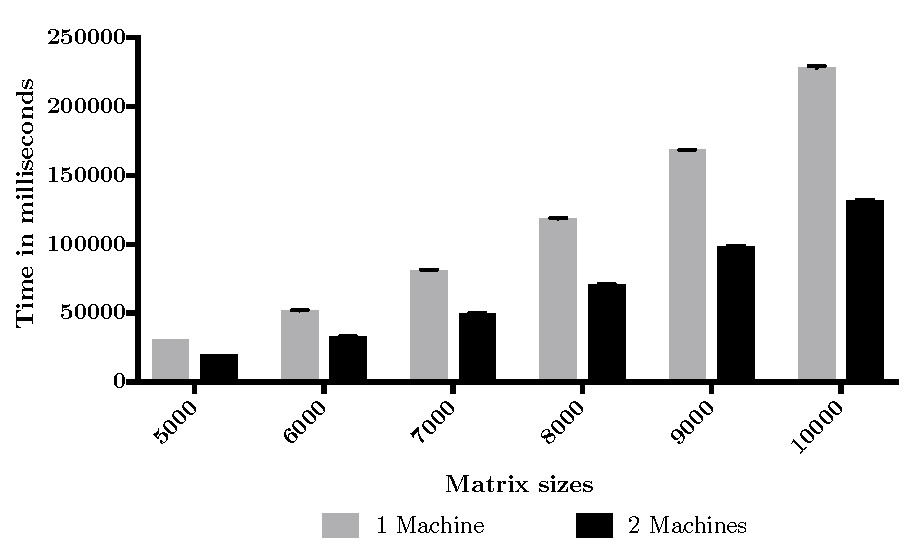
\includegraphics[width=1.0\textwidth]{images/sharded_matrix_multi.pdf}
	\centering
	\caption{Parallel Matrix Multiplication}
	\label{img:parallel_matrix}
\end{figure}

Figure \ref{img:parallel_matrix} shows that using an additional machine can lead to substantial performance benefits. It is visible that for small problem sizes the speedup is only marginal between 10-30\%. This is due to the fact that for the smaller matrix sizes the computations are executed relatively fast but are neutralized by the network interconnect that has to serve both machines at the same time. For larger matrices the ratio of computation to transferred data becomes smaller thus diminishing the network congestion effect. This can be reasoned as with rising matrix sizes of $n^2$ the computational complexity increases by $n^3$. It also becomes apparent that with growing problem sizes the speedup gets greater with a decreasing slope, which indicates that it hits a barrier around 75\%. This barrier might be imposed due to overheads by Dynamic OpenCL, Aparapi and dOpenCL but may be mainly the result of network congestions.

As matrix multiplications are computations that require noticeable amounts of data that influence the overall performance through network transfers, a second type of computation shall be evaluated that has very low data requirements. Such a workload is the Mandelbrot set, which does not need initial data but computes values according to positions in a two dimensional array. The Mandelbrot set was executed just as the previous matrix multiplication with 5 runs per problem size.

\begin{figure}[H]
	
	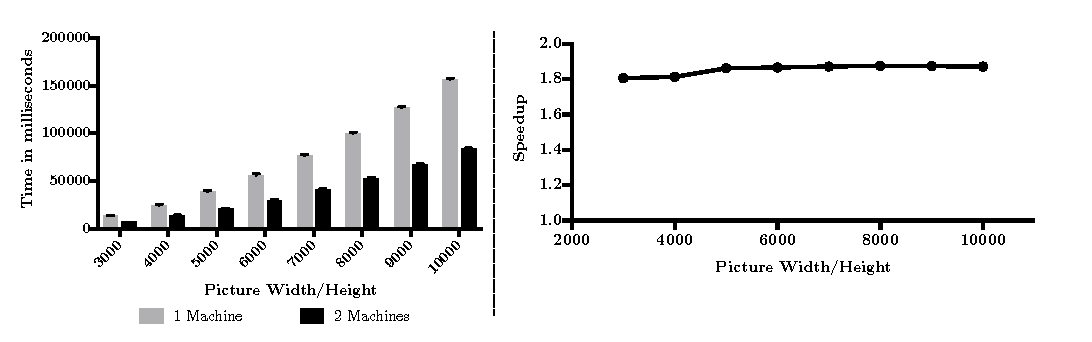
\includegraphics[width=1.0\textwidth]{images/sharded_mandelbrot.pdf}
	\centering
	\caption{Parallel Mandelbrot}
	\label{img:parallel_mandelbrot}
\end{figure}

Figure \ref{img:parallel_mandelbrot} reveals that its low data transfer requirements severely benefit the performance speedup. With speedups between 80\% and 88\% the maximum increase in performance is not only significantly higher than for the matrix multiplications but is also more stable in correlation to the problem sizes.


\subsection{Job Suite Performance}
\label{job_suite_performance}

Section \ref{single_job_performance} identified benefits when utilizing Dynamic OpenCL for a single job. In order to simulate a shared cluster environment it becomes necessary to evaluate its performance by executing variety of parallel jobs. For this reason a job suite was compiled that comprises six workloads of various complexity and type. Not only should the runtime differ per Kernel of each job but also their transferable data. The list of workloads is shown in table \ref{table:benchmark_job_setup} with the respective abbreviated identifiers that are used throughout the chapter.

\begin{table}[!htb]
	\centering
	\begin{adjustbox}{width=0.95\textwidth}
		\small
		\begin{tabular}{l | l | l | l | l}
			~ & \textbf{Abbreviation}						& \textbf{Computational Effort}		& \textbf{Iterations}	& \textbf{Kernels per Iteration} \\
			\hline
			\textbf{Matrix Multiplication 1}	& MM1  	& 8000x8000  								& 1 	& 5 \\
			\textbf{Matrix Multiplication 2} 	& MM2	& 6000x6000  								& 1		& 5 \\
			\textbf{Mandelbrot 1}     		 	& MB1	& 1000x1000 (1000000 iterations per point) 	& 1		& 5 \\
			\textbf{Mandelbrot 2}				& MB2	& 2000x2000 (600000 iterations per point)  	& 1		& 5 \\
			\textbf{K-means}          			& KM 	& 6000000 objects and 200 clusters  		& 10	& 1 \\
			\textbf{N-body}    		 			& NB 	& 64000 objects  							& 10	& 1 \\		
		\end{tabular}
	\end{adjustbox}
	
	\caption{Benchmark Job Setup}
	\label{table:benchmark_job_setup}
\end{table}

The set of workloads thus comprises a mix of iterative and non-iterative tasks. While the iterative jobs have a fixed number of iterations and are not split per round, non-iterative tasks are split into 5 parts to enable parallelization. Although some jobs employ the same algorithm, the problem sizes are varied to create a more heterogeneous set. The implications of the problem sizes and splits for each job are explained in section \ref{workload_explanation}.

In order to prove the heterogeneity of the supplied workloads in terms of computational complexity and data transfer properties, analytical test runs are executed on a local machine of class B that measure the execution time per Kernel and the transfered data sizes. The following figure display the results of running the suite five times:

\begin{figure}[H]
	
	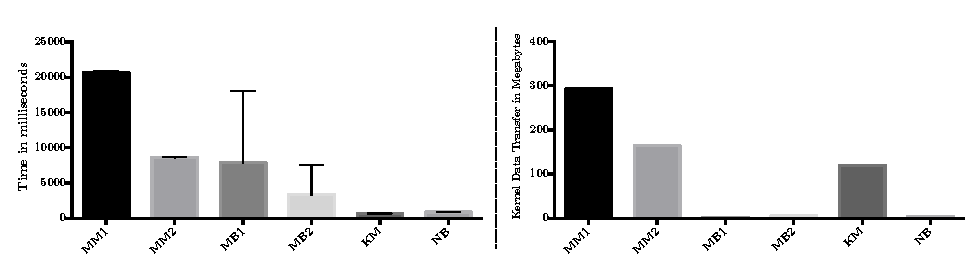
\includegraphics[width=1.0\textwidth]{images/benchmark_kernel_data_transfers.pdf}
	\centering
	\caption{Average Kernel Runtimes and Data Transfer Sizes}
	\label{img:benchmark_kernel_attributes}
\end{figure}

While it is visible that the computation times are very different, it can also be seen that the respective data transfers do not correlate to that attribute. For example, while MM2 and MB1 may require similar execution times, MM2 transfers 100x more data than MB1. The same is true for the iterative jobs KM and NB. It must be noted that MB1 and MB2 show a great standard deviation, which are not measurement errors but are a result of the nature of the algorithm. Mandelbrot calculations can not be split evenly in terms of computational effort and instead may run some Kernels for long times while having virtually no computations required by other Kernels.

For the benchmark the performance indicator to measure is the total time to finish all tasks. As the selection of scheduling algorithms has a big impact on this value, it is necessary to define the utilized algorithms. For the job scheduling tier a round robin approach is used. On the device scheduling level a historic performance based algorithm is used that assigns a Kernel to the best performing device in case multiple are available. In order to allow for a fair comparison among multiple runs, all jobs are submitted before starting the execution engine.

The suite is executed five times on three different cluster setups. At first it is executed on a single machine of class B. In this setup no network transfer is needed as the management node also executed the Kernels. For the second cluster a machine of class B is added, which is connected by a 10 Gbit/s interconnect. Therefore, some Kernels may have to be sent over the network while others will be executed directly on the management node. In the final run another machine of class A is added, which is only connected with 1 Gbit/s but has a very high computational capability. The results of the benchmark are visible in the following figure:

\begin{figure}[H]
	
	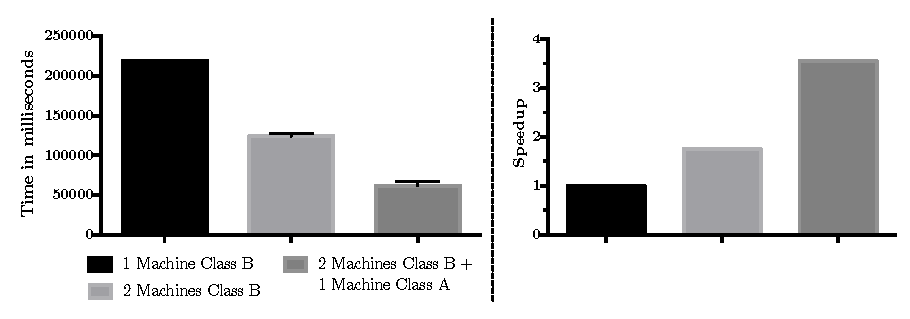
\includegraphics[width=1.0\textwidth]{images/local_full_benchmark_results.pdf}
	\centering
	\caption{Local Benchmark Results}
	\label{img:local_benchmark_results}
\end{figure}

The results indicate that employing a second machine that is connected through a fast Ethernet connection can produce significant performance benefits. Although Kernels have to be sent over the network to the second machine, it still yields an average speedup of x1.76. It also reveals that the scheduling works sufficiently even though it is based on naive algorithms. In the last cluster setup the high performance machine of class A is added, which is connected only by 1 Gbit/s. Even though the network slows down the execution times on this machine it can still double the performance of the cluster, leading to a speedup of x3.54. Thus it can be concluded that the parallelization by Dynamic OpenCL through remote machines is a viable option within a shared local cluster. It has to be noted though that high performance machines like machines of class A may be underutilized and slowed down by network transfers.

\section{Hybrid Distribution}

After having discussed the benefits of local workload distributions, it is necessary to evaluate the performance of Dynamic OpenCL when connected to cloud resources. For this, the benchmarks used in \ref{local_distribution} are applied to a cluster that holds local machines as well as resources that are booked on the Amazon EC2 cloud. In the setup only a single local machine of class B is employed. It serves as a management node as well as an execution node. 

For the cloud resources a high performance computation instance type is chosen: the c4.8xlarge instances provide 36 Intel Xeon E5-2666 v3 cores at 2.9 GHz as well as 60 GB of RAM. Amazon also promises to connect these instances through 10 Gbit/s interconnects.

While 10 Gbit/s interconnects proved to be a very potent solution when distributing among a local cluster, hybrid clusters suffer from far slower bottlenecks in between the two networks. The local cluster is set in Potsdam and should therefore be connected to the geographically closest region that is available on the EC2 cloud, which is in Frankfurt. As a first measure the interconnection speed between the two locations is measured by using iperf and ping from the local machine to a cloud machine over a minute. Then the same is done from a another c4.8xlarge machine within the EC2. The following table shows the network performance results:

\begin{table}[!htb]
	\centering
	\begin{adjustbox}{width=0.5\textwidth}
		\small
		\begin{tabular}{l | l | l}
			~                     & Local                 				& Remote                  \\
			\hline
			iperf3                & 2.69 Gbit/s ($\sigma = 0.05$) 		& 169.26 Mbit/s ($\sigma = 11.93$) \\
			ping                  & 0.317 ms ($\sigma = 0.037$)  		& 18.9 ms ($\sigma = 0.17$)  \\
		\end{tabular}
	\end{adjustbox}
	
	\caption{Local vs. Remote interconnection EC2}
	\label{table:local_vs_remote_ec2}
\end{table}

While machines within EC2 may profit from fast network connections, accessing the same machines remotely from a local cluster offers significantly higher latencies and lower bandwidths. A reason for the low remote performance numbers could be bottlenecks within the local network that reduce the bandwidth significantly. In order to investigate this theory three machines of type c4.8xlarge. Then a single local machine launches iperf3 tests for 60 seconds in parallel to each of the three machines. The results are shown in the following figure:

\begin{figure}[H]
	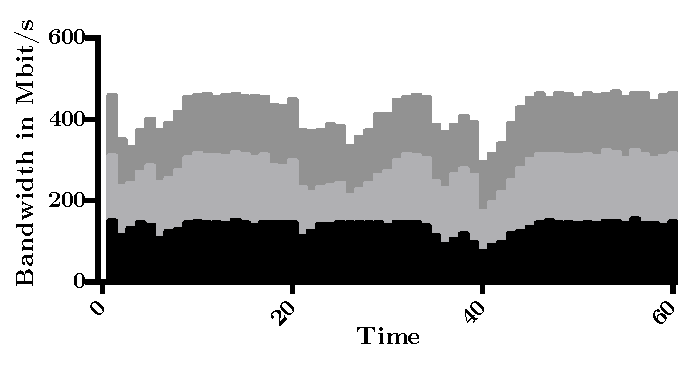
\includegraphics[width=0.5\textwidth]{images/ec2_stacked_network_performance.pdf}
	\centering
	\caption{EC2 Parallel Network Performance}
	\label{img:EC2 Parallel Network Performance}
\end{figure}

It is visible that the total network performance reaches 480 MBit/s in total for some data points, which disproves that the bottleneck lies within the local network. Instead it appears as if the EC2 only provides limited network capabilities per instance when accessed from outside of their cluster.

\subsection{Single Job Performance}

Similar to the benchmarks conducted in \ref{single_job_performance}, matrix multiplication and Mandelbrot sets of differing sizes are computed first on a single local machine and then on an additional c4.8xlarge instance.

\begin{figure}[H]
	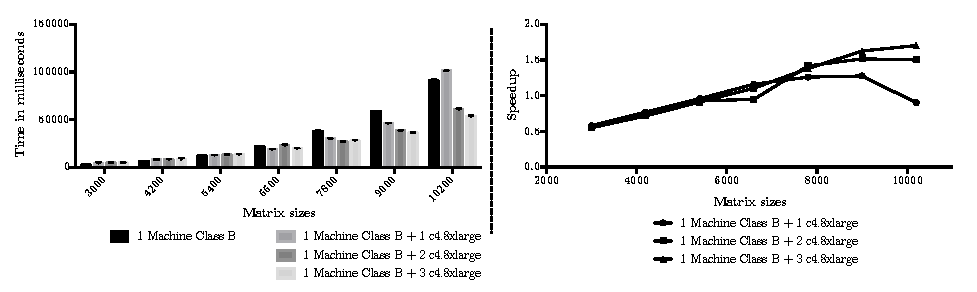
\includegraphics[width=1.0\textwidth]{images/hybrid_matrix_multiplication.pdf}
	\centering
	\caption{Hybrid Matrix Multiplication}
	\label{img:hybrid_matrix_multiplication}
\end{figure}

Figure \ref{img:hybrid_matrix_multiplication} displays the results for the matrix multiplications. It is visible that adding a cloud computation device for this workload adds only marginal performance improvements or even slows down the process in the case of smaller problem sizes. With increasing sizes the performance benefits become significant, peaking at around 50\% for the largest measured size. Even the 50\% increase in performance is not very promising as the c4.8xlarge instance brings in 36 additional cores and should therefore add much more computational capabilities to the already employed 8 cores of the local class B machine. As the connection between both networks is much slower than the typical bus speeds of the c4.8xlarge, it mainly remains underutilized due to the increased transfer times.


\begin{figure}[H]	
	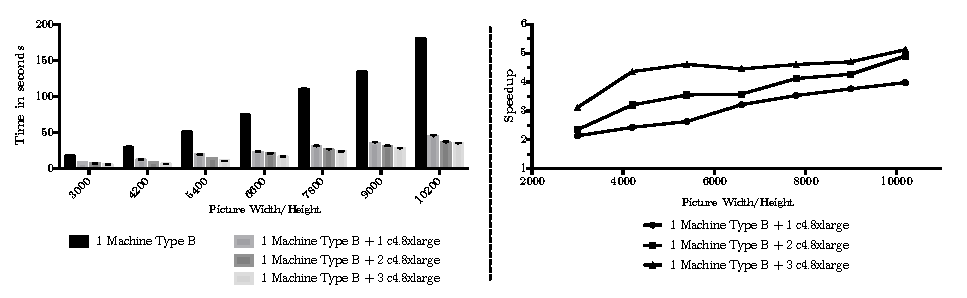
\includegraphics[width=1.0\textwidth]{images/hybrid_mandelbrot_performance.pdf}
	\centering
	\caption{Hybrid Mandelbrot Set}
	\label{img:hybrid_mandelbrot}
\end{figure}


For the second benchmark the Mandelbrot set is used again, which promises better performance than matrix multiplications on a hybrid setup due to its lower data requirements. The results of the measurements are shown in figure \ref{img:hybrid_mandelbrot}. In fact the c4.x8large can greatly improve the overall system performance through its 36 cores. Even for small problem sizes it already provides significant benefits but especially for the larger sizes it can speed up the execution by around x2.5. Thus it is concluded that the data requirements of a workload have an even greater impact on performance for hybrid setups than on an entirely local setup.

\subsection{Job Suite Performance}

In order to simulate a shared hybrid cluster environment the same tests as in section \ref{job_suite_performance} are conducted. That means that the equal selection of jobs is submitted to the cluster, which consists of a single local machine of class B. This machine serves for management and execution in parallel. The cloud resources are comprised of a variable number of c4.8xlarge instances provided by Amazon. Again, for scheduling a Round Robin approach paired with the historical performance based device scheduler is utilized.

\begin{figure}[H]	
	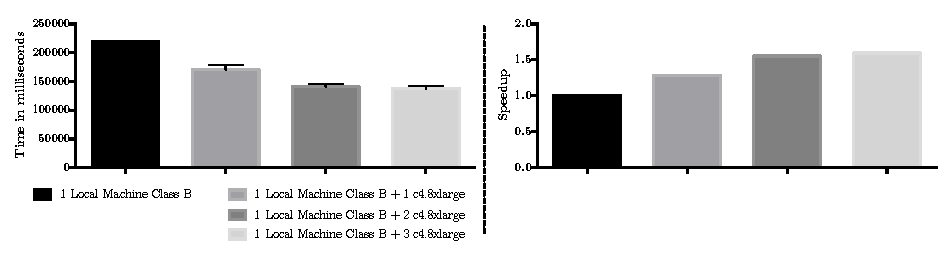
\includegraphics[width=1.0\textwidth]{images/hybrid_full_benchmark_performance_based.pdf}
	\centering
	\caption{Hybrid Benchmark Results}
	\label{img:hybrid_benchmark_results}
\end{figure}

Figure \ref{img:hybrid_benchmark_results} shows the results of the benchmark with various numbers of cloud resources. It is visible that the performance benefits are quite insignificant in relation to the potential computational capability of the c4.8xlarge instance types. Scaling the cluster to two machines with one c4.8xlarge gives a 28\% performance increase. Adding another c4.8xlarge instance grants an overall 55\% faster execution compared to the single local machine. When a third instance is introduced, it becomes obvious that a barrier is hit for this benchmark as the speedup compared to two cloud machines is minimal. As shown earlier the EC2 offers low network bandwidth when accessed by the local cluster. While the performance based scheduler can take these factors into account through its history based approach it still has to run a partial of a job at least once to gain a performance measurement. Therefore tasks with big data transfers may be assigned several times to different cloud machines, thus resulting in slow execution times for these Kernels. 

In order to optimize the assignment of data intense jobs to the appropriate devices a new scheduler is built that has awareness of the different network locations. For this all available devices are marked whether they are originating from the local cluster or the cloud provider. The scheduler then ignores the task order given by the first scheduling tier, e.g. Round Robin, and imposes its own order. In fact it sorts the assignable Kernels by the amount of data they are comprised of and assigns them from either end: cloud devices receive tasks with little data while local devices are assigned Kernels with the biggest data sizes. Thus tasks should reach cloud devices much faster and the scheduling is not reliant on historical data anymore. With the new scheduler the benchmark is executed again.

\begin{figure}[H]	
	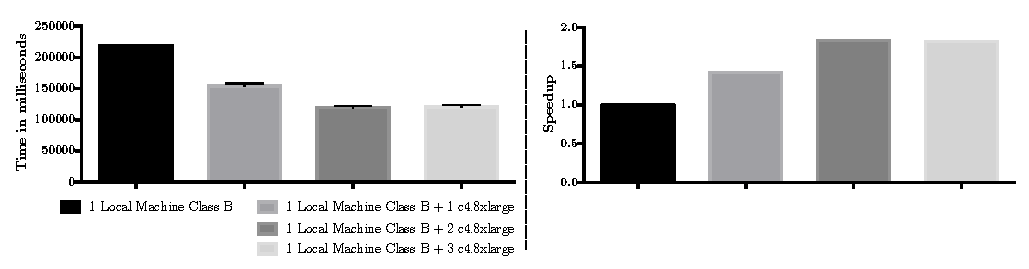
\includegraphics[width=1.0\textwidth]{images/hybrid_full_benchmark_network_based.pdf}
	\centering
	\caption{Hybrid Benchmark Results (Network Aware Scheduler)}
	\label{img:hybrid_benchmark_results_network_aware}
\end{figure}

Figure \ref{img:hybrid_benchmark_results_network_aware} shows that the new scheduler introduces noticeable benefits compared to the historical performance based approach. While a single c4.8xlarge instance improves the system performance by 42\%, adding another one leads to a 83\% increase. Compared to 28\% and 55\% respectively for the performance based scheduler this depicts a significant improvement even though the new mechanism is very basic. When a third c4.8xlarge machine is introduced to the cluster no further speedup can be achieved for this workload.

